\documentclass{article}

\usepackage{amsfonts, amsmath,amssymb,amsthm}   % Paquetes de simbología matemática básica
\usepackage{lmodern,microtype,bm}     % Fuente y espaciado entre letras; lo deja bonito
\usepackage{dsfont, graphicx}
\usepackage{mathrsfs, halloweenmath,xcolor}
\usepackage{MnSymbol}
\usepackage{mathtools}
\usepackage{multicol,titlesec}
\usepackage[shortlabels]{enumitem}    % Continuar listas en mini-páginas distintas
\usepackage{physics}
\usepackage[english,spanish]{babel}   % Cambia los comandos de texto predeterminados (capítulos, 			                                        secciones, bibliografía, etc.) a español
\decimalpoint
\usepackage[style=mexican]{csquotes}  % Comillas y otros elementos de citación
\textwidth 16cm                       % Ancho
\oddsidemargin -0.0cm                 % Espacio de margen (como es formato de libro, los margenes se 		                                        declaran para páginas pares e impares
\usepackage[spanish]{todonotes}
\usepackage{xfrac}
\usepackage[unicode=true]{hyperref}

\newtheoremstyle{definicion}% name
{3pt}% Space above
{3pt}% Space below
{}% Body font
{}% Indent amount
{\color{blue}\bfseries}% Theorem head font
{.}% Punctuation after theorem head
{.5em}% Space after theorem head
{}%
\theoremstyle{definicion}
\newtheorem{definicion}{Def.}

\theoremstyle{definition}             % Con el paquete amsmath se pueden personalizar los estilos de
\newtheorem*{inst}{Instrucciones}

\theoremstyle{definition}             % Con el paquete amsmath se pueden personalizar los estilos de
\newtheorem{sol}{Solución}

\theoremstyle{definition}
\newtheorem{record}{Recordatorio}

\theoremstyle{definition}
\newtheorem{properties}{Propiedades}

\newtheoremstyle{observacion}% name
{3pt}% Space above
{3pt}% Space below
{}% Body font
{}% Indent amount
{\color{red}\bfseries}% Theorem head font
{.}% Punctuation after theorem head
{.5em}% Space after theorem head
{}%
\theoremstyle{observacion}
\newtheorem{obs}{Obs.}

\theoremstyle{definition}
\newtheorem{prop}{Proposición}

\theoremstyle{plain}
\newtheorem{lemma}{Lema}
\newtheorem{theorem}{Teorema}

\theoremstyle{definition}
\newtheorem{exe}{Ejemplo}

\newtheoremstyle{afirmacion}% name
{3pt}% Space above
{3pt}% Space below
{}% Body font
{}% Indent amount
{\color{green!40!black}\bfseries}% Theorem head font
{.}% Punctuation after theorem head
{.5em}% Space after theorem head
{}%
\theoremstyle{afirmacion}
\newtheorem{corollary}{Corolario}

\newtheoremstyle{notation}% name
{3pt}% Space above
{3pt}% Space below
{}% Body font
{}% Indent amount
{\color{magenta}\bfseries}% Theorem head font
{.}% Punctuation after theorem head
{.5em}% Space after theorem head
{}%
\theoremstyle{notation}
\newtheorem{notation}{Notación}

\theoremstyle{definition}
\newtheorem{eje}{Ejercicio}

\setlength{\parindent}{2em}           % Sangría
\setlength{\parskip}{0.5em}           % Espacio entre párrafos

\graphicspath{{./img}}
\DeclareMathOperator*{\ang}{\overrightarrow{\textrm{ang}}}

\title{\Huge{El plano euclidio}}
\author{Geometría Analítica I}
\date{\today}

\begin{document}
    \maketitle

    \section{El espacio vectorial \texorpdfstring{\(\mathbb{R}^{2}\)}{ℝ²}}

    En esta sección se introduce la herramienta algebraica básica para hacer geometría con parejas, ternas o \(n\)-adas de números.

    \begin{definicion}
        Dados dos vectores \(\vb*{u} = (x, y)\) y \(\vb{v} = (x^{\prime}, y^{\prime})\) en \(\mathbb{R}^{2}\), definimos su \textcolor{blue}{suma vectorial}, o simplemente suma, como el vector \(\vb*{u} + \vb*{v}\) que resulta de sumar componente a componente:

        \begin{equation*}
            \vb*{u} + \vb*{v} \coloneq (x + x^{\prime}, y + y^{\prime}).
        \end{equation*}

        Nótese que en cada coordenada, la suma que se usa es la suma usual de números reales.
    \end{definicion}

    La suma vectorial corresponde geométricamente a la regla del paralelogramo usada para encontrar la resultante de dos vectores. Esto es, se consideran los vectores como segmentos dirigidos que salen del origen y generan entonces un paralelogramo, y el vector que va del origen a la otra esquina es la suma.
    
    \begin{figure}[htb]
        \centering
        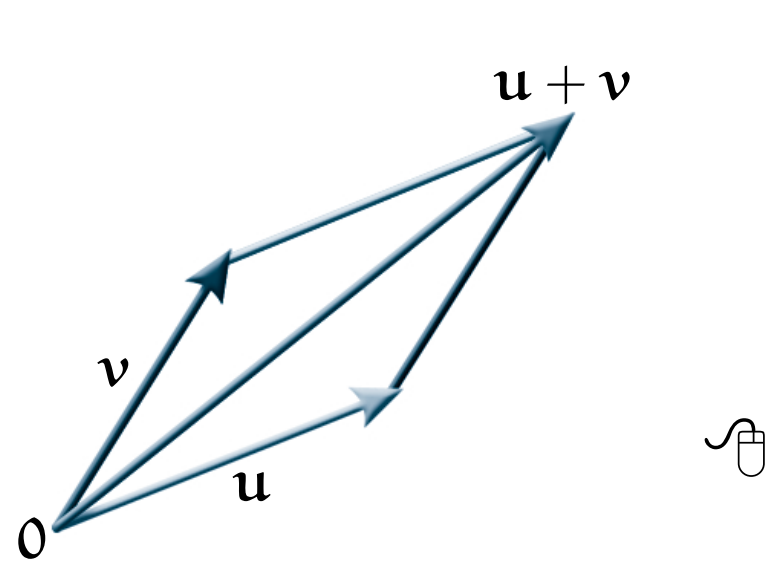
\includegraphics[scale=0.2]{1}
        \caption{Método del paralelogramos}
        \label{fig:paralelogramo}
    \end{figure}

    \begin{definicion}
        Dados un vector \(\vb*{u} = (x, y) \in \mathbb{R}^{2}\) y un número \(t \in \mathbb{R}\) se define la \textcolor{blue}{multiplicación escalar} \(t \vb*{u}\) como el vector que resulta de multiplicar cada componente del vector por el número:

        \begin{equation*}
            t \vb*{u} \coloneq (t x, t y).
        \end{equation*}

        Nótese que en cada coordenada la multiplicación que se usa es de los números reales.
    \end{definicion}

    \begin{obs}
        Notemos que \(t \vb*{u}\) para \(t > 1\) es, estrictamente hablando, una \textcolor{blue}{dilatación} de \(\vb*{u}\), y para \(0 < t < 1\), una \textcolor{blue}{contracción} del mismo. Además, para \(t < 0\), \(t \vb*{u}\) apunta en la dirección contraria, ya que, en particular, \((-1) \vb*{u} \eqqcolon - \vb*{u}\) es el vector que, como segmento dirigido, va del punto \(\vb*{u}\) al \(\vb*{0}\) y el resto se obtiene como dilataciones o contracciones de \(- \vb*{u}\).
    \end{obs}

    Las propiedades básicas de la suma vectorial y la multiplicación escalar se reúnen en el siguiente teorema, donde el vector \(\vb*{0} = (0, \dots, 0)\) es el llamado \textcolor{blue}{vector cero} que corresponde al origen, y, para cada \(x \in \mathbb{R}^{n}\), el vector \(-x \coloneq (-1)x\) se llama \textcolor{blue}{inverso aditivo} de \(x\).

    \begin{theorem}
        Para todos los vectores \(x,\ y,\ z \in \mathbb{R}^{n}\) y para todos los números \(s,\ t \in \mathbb{R}\) se cumple que:

        \begin{enumerate}[label = \textnormal{\Roman*)}]
            \item \((x + y) + z = x + (y + z)\)
            \item \(x + y = y + z\)
            \item \(x + \vb*{0} = x\)
            \item \(x + (-x) = \vb*{0}\)
            \item \(s(tx) = (st)x\)
            \item \(1x = x\)
            \item \(t(x + y) = tx + ty\)
            \item \((s + t)x = sx + tx\)
        \end{enumerate}
    \end{theorem}

    \begin{lemma}
        Si \(x \in \mathbb{R}^{2}\) y \(t \in \mathbb{R}\) son tales que \(tx = \vb*{0}\) entonces \(t = 0\) 0 \(x = \vb*{0}\).
    \end{lemma}

    \section{Líneas}

    Se nos pide describir el conjunto \(\mathcal{L}_{\vb*{v}} \coloneq \left\lbrace t\vb*{v} \in \mathbb{R}^{2} \mid t \in \mathbb{R}\right\rbrace\) donde \(\vb*{v} \in \mathbb{R}^{2}\). Es claro que que si \(\vb*{v} \neq \vb*{0}\), entonces \(\mathcal{L}_{\vb*{v}}\), al constar de todos los múltiplos escalares del vector \(\vb*{v}\), se dibuja como una recta que pasa por el origen (pues \(\vb*{0} = 0\vb*{0}\)) con la dirección de \(\vb*{v}\).

    \begin{definicion}
            Dados un punto \(\vb*{p}\) y un vector \(\vb*{v} \neq \vb*{0}\), la \textcolor{blue}{recta que pasa por} \(\vb*{p}\) \textcolor{blue}{con dirección} \(\vb*{v}\) es el conjunto

            \begin{equation*}
                \ell \coloneq \left\lbrace \vb*{p} + t\vb*{v} \mid t \in \mathbb{R}\right\rbrace.
            \end{equation*}

            Una \textcolor{blue}{recta} o \textcolor{blue}{línea} en \(\mathbb{R}^{2}\) es un subconjunto que tiene, para algún \(\vb*{p}\) y \(\vb*{v} \neq \vb*{0}\), la descripción anterior.
            A esta forma de definir una recta se le conoce como \textcolor{blue}{representación (o expresión) paramétrica}.
    \end{definicion}

    \begin{lemma}
        Dados dos puntos \(\vb*{p}\) y \(\vb*{q}\) en \(\mathbb{R}^{2}\), existe una recta que pasa por ellos.
    \end{lemma}
    \begin{proof}
        Si tuviéramos que \(\vb*{p} = \vb*{q}\), como  hay muchas rectas que pasan por \(\vb*{p}\), ya acabamos. Supongamos entonces que \(\vb*{p} \neq \vb*{q}\). Si tomamos a \(\vb*{p}\) como punto base para la recta que buscamos, bastará con encontrar un vector que nos lleve de \(\vb*{p}\) a \(\vb*{q}\), para tomarlo como dirección. Este es la diferencia \(\vb*{q} - \vb*{p}\), pues claramente

        \begin{equation*}
            \vb*{p} + (\vb*{q} - \vb*{p}) = \vb*{q},
        \end{equation*}

        de tal manera que si definimos \(\vb*{d} \coloneq \vb*{q} - \vb*{p}\), como dirección, la recta

        \begin{equation*}
            \ell \coloneq \left\lbrace \vb*{p} + t\vb*{d} \mid t \in \mathbb{R}\right\rbrace
        \end{equation*}

        (que sí es una recta pues \(\vb*{d} = \vb*{q} - \vb*{p} \neq \vb*{0}\)), es la que funciona. Con \(t = 0\) obtenemos que \(\vb*{p} \in \ell\), y con \(t = 1\) que \(\vb*{q} \in \ell\).
    \end{proof}

    \begin{obs}
        Obsérvese que cuando \(t\) toma valores entre \(0\) y \(1\), se obtienen puntos entre \(\vb*{p}\) y \(\vb*{q}\), así que al \textcolor{blue}{segmento} de \(\vb*{p}\) a \(\vb*{q}\), que denotaremos con \(\overline{\vb*{p}\vb*{q}}\), se debe definir como

        \begin{equation*}
            \overline{\vb*{p}\vb*{q}} \coloneq \left\lbrace \vb*{p} + t(\vb*{p} - \vb*{q}) \mid 0 \leq t \leq 1\right\rbrace.
        \end{equation*}

        Y la recta \(\ell\) que pasa por \(\vb*{p}\) y \(\vb*{q}\) se extiende ``indefinidamente'' a ambos lados del segmento \(\overline{\vb*{p}\vb*{q}}\), para \(t > 1\) del lado de \(\vb*{q}\) y para \(t < 0\) del lado de \(\vb*{p}\).
    \end{obs}

    \subsection{Coordenadas baricéntricas}

    Supongamos que \(\vb*{p}\) y \(\vb*{q}\) son puntos distintos del plano. Para cualquier \(t \in \mathbb{R}\) , se tiene que

    \begin{equation*}
        \vb*{p} + t(\vb*{q} - \vb*{p}) = \vb*{p} + t\vb*{q} - t\vb*{p} = (1 - t)\vb*{p} + t\vb{q}
    \end{equation*}

    al reagrupar los términos. Y esta última expresión, a su vez, se puede reescribir como 

    \begin{equation*}
        s\vb*{p} + t\vb*{q}\quad \text{con} \quad s + t = 1,
    \end{equation*}

    donde hemos introducido la nueva variable \(s = 1 - t\). De lo anterior se deduce que la recta \(\ell\) que pasa por \(\vb*{p}\) y \(\vb*{q}\) puede también describirse como 

    \begin{equation*}
        \ell \coloneq \left\lbrace s\vb*{p} + t\vb*{q} \mid s + t = 1\right\rbrace,
    \end{equation*}

    que es una \textcolor{blue}{expresión baricéntrica} de \(\ell\). A los números \(s,\ t\) se les conoce como \textcolor{blue}{coordenadas baricéntricas} del punto \(x = s\vb*{p} + t\vb*{q}\).

    Las coordenadas baricéntricas tienen la ventaja de que ya no distinguen entre los dos puntos. Al expresar una recta en coordenadas baricéntricas no le damos una dirección preferida. Se usan simultáneamente los parámetros naturales para las dos direcciones (de \(\vb*{p}\) a \(\vb*{q}\) y de \(\vb*{q}\) a \(\vb*{p}\)); pues si \(s + t = 1\), entonces

    \begin{equation*}
        s\vb*{p} + t\vb*{q} = \vb*{p} + t(\vb*{q} - \vb*{p}) = \vb*{q} + s(\vb*{p} - \vb*{q}).
    \end{equation*}

    Nótese que \(x = s\vb*{p} + t\vb*{q}\) está en el segmento entre \(\vb*{p}\) y \(\vb*{q}\) si y solo si \(t \geq 0\) y \(s \geq 0\). La extensión de la recta más allá de \(\vb*{q}\) tiene coordenadas baricéntricas \(s,\ t\) con \(s < 0\) (y por lo tanto \(t > 1\)); así que los puntos de \(\ell\) fuera del segmento de \(\vb*{p}\) a \(\vb*{q}\) tienen alguna coordenada baricéntrica negativa (la correspondiente al punto más lejano).

    \begin{theorem}[De las medianas]
        Dado un triángulo \(\vb*{a},\ \vb*{b}\) y \(\vb*{c}\), sus tres medianas ``concurren'' en un punto que las parte en la proporción \(\frac{2}{3}\) a \(\frac{1}{3}\) (del lado opuesto).

        \missingfigure[]{Insertar figura del teorema que se encuentra en la página 38}
    \end{theorem}

    \begin{proof}
        Puesto que el punto medio del segmento \(\vb*{b},\ \vb*{c}\) es (\(\frac{1}{2}\vb*{b} + \frac{1}{2}\vb*{c}\)), entonces la mediana por \(\vb*{a}\) es el segmento

        \begin{equation*}
            \left\lbrace s\vb*{a} + t \left(\dfrac{1}{2}\vb*{b} + \dfrac{1}{2}\vb*{c}\right) \mid s + t = 1,\ s, t \geq 0\right\rbrace,
        \end{equation*}

        y análogamente se describen las otras dos medianas. Por suerte, el enunciado del teorema nos dice dónde buscar la intersección: el punto que describe en la mediana de \(\vb*{a}\) es precisamente

        \begin{equation*}
            \dfrac{1}{3}\vb*{a} + \dfrac{2}{3}\left(\dfrac{1}{2}\vb*{b} + \dfrac{1}{2}\vb*{c}\right) = \dfrac{1}{3}\vb*{a} + \dfrac{1}{3}\vb*{b} + \dfrac{1}{3}\vb*{c}.
        \end{equation*}

        Entonces, de las igualdades se deduce que las tres medianas \emph{concurren} en el punto \(\frac{1}{3}(\vb*{a} + \vb*{b} + \vb*{c})\), es decir, pasan por él. Este punto se llama el \textcolor{blue}{baricentro} del triángulo, y claramente parte a las medias en la proporción deseada. De nuevo, el baricentro corresponde al ``centro de masa'' o ``punto de equilibrio'' del triángulo.
    \end{proof}

    \subsection{Planos en el espacio I}

    % En el teorema de las medianas se usó una idea que nos sirve para definir planos en el espacio. Dados tres puntos \(\vb*{a},\ \vb*{b}\) y \(\vb*{c}\) en \(\mathbb{R}^{3}\), ya sabemos describir las tres líneas entre ellos; supongamos que son distintas. Entonces podemos tomar nuevos puntos en alguna de ellas y de estos las nuevas líneas que los unen al vértice restante. Está claro que la unión de todas estas líneas debe ser el plano que pasa por \(\vb*{a},\ \vb*{b}\) y \(\vb*{c}\).

    % Un punto \(y\) en la línea que pasa por \(\vb*{a}\) y \(\vb*{b}\) se escribe como

    % \begin{equation*}
    %     y = s\vb*{a} + t\vb*{b}\quad \text{con}\quad s + t = 1.
    % \end{equation*}

    % Y un punto \(x\) en la línea que pasa por \(y\) y \(\vb*{c}\) se escribe entonces como

    % \begin{equation*}
    %     x = r(s\vb*{a} + t\vb*{b}) + (1 - t)\vb*{c},
    % \end{equation*}

    % para algún \(r \in \mathbb{R}\); que es lo mismo que

    % \begin{equation*}
    %     x = (rs)\vb*{a} + (rt)\vb*{b} + (1 - t)\vb*{c}.
    % \end{equation*}

    % \missingfigure[]{Insertar figura correspondiente a la introducción de la subsección en la página 39}

    % Observemos que los tres coeficientes suman uno:

    % \begin{equation*}
    %     (rs) + (rt) + (1 - r) = r(s + t) + 1 - r = r(1) + 1 - r = 1.
    % \end{equation*}

    % Demostraremos que está en una línea por uno de los vértices y un punto en la línea que pasa por los otros dos.
    % Sean \(\alpha,\ \beta,\ \gamma \in \mathbb{R}\) tales que \(\alpha + \beta + \gamma = 1\). Consideremos el punto

    % \begin{equation*}
    %     x = \alpha\vb*{a} + \beta\vb*{b} + \gamma\vb*{c}.
    % \end{equation*}

    % Como alguno de los coeficientes es distinto de \(1\), podemos suponer sin pérdida de generalidad que \(\alpha \neq 1\). Entonces podemos dividir entre \(1 - \alpha\) y se tiene
    
    % \begin{equation*}
    %     x = \alpha\vb*{a} + (1 - \alpha)\left(\dfrac{\beta}{1 - \alpha}\vb*{b} + \dfrac{\gamma}{1 - \alpha}\vb*{c}\right),
    % \end{equation*}

    % así que \(x\) está en la recta que pasa por \(\vb*{a}\) y el punto

    % \begin{equation*}
    %     y = \dfrac{\beta}{1 - \alpha}\vb*{b} + \dfrac{\gamma}{1 - \alpha}\vb*{c}.
    % \end{equation*}

    % Como \(\alpha + \beta + \gamma = 1\), entonces \(\beta + \gamma = 1 - \alpha\), y los coeficientes de esta última expresión suman uno. Por lo tanto \(y\) está en la recta que pasa por \(\vb*{b}\) y \(\vb*{c}\).

    \begin{definicion}
        Dados tres puntos \(\vb*{a},\ \vb*{b}\) y \(\vb*{c}\) en \(\mathbb{R}^{3}\) no colineales (es decir, que no estén en una misma línea), el \textcolor{blue}{plano afín} que pasa por ellos es el conjunto

        \begin{equation*}
            \Pi = \left\lbrace \alpha\vb*{a} + \beta\vb*{b} + \gamma\vb*{c} \mid \alpha, \beta, \gamma \in \mathbb{R}; \alpha + \beta + \gamma = 1\right\rbrace.
        \end{equation*}
    \end{definicion}

    \begin{obs}
        A una expresión de la forma \(\alpha\vb*{a} + \beta\vb*{b} + \gamma\vb*{c}\) con \(\alpha + \beta + \gamma = 1\) la llamaremos \textcolor{blue}{combinación afín} (o \textcolor{blue}{baricéntrica}) de los puntos \(\vb*{a},\ \vb*{b}\) y \(\vb*{c}\) y los coeficientes \(\alpha,\ \beta,\ \gamma\), las \textcolor{blue}{coordenadas baricéntricas} del punto \(\alpha\vb*{a} + \beta\vb*{b} + \gamma\vb*{c}\). 
    \end{obs}

    \subsubsection*{Definición lineal}

    La recta que genera un vector \(\vb*{u} \neq \vb*{0}\) es el conjunto de todos sus ``alargamientos'' \(\mathcal{L}_{\vb*{u}} = \left\lbrace s\vb*{u} \mid s \in \mathbb{R}\right\rbrace\). Si ahora tomamos un nuevo vector \(\vb*{v}\) que no esté en \(\mathcal{L}_{\vb*{u}}\), tenemos una nueva recta \(\mathcal{L}_{\vb*{v}} = \left\lbrace t\vb*{v} \mid t \in \mathbb{R}\right\rbrace\) que intersecta a la anterior solo en el origen. Estas dos rectas generan un plano que consiste en todos los puntos a los cuales se pueden llegar desde el origen moviéndose únicamente en las direcciones \(\vb*{u}\) y \(\vb*{v}\). Este plano que pasa por el origen claramente se describe con dos parámetros independientes:

    \begin{equation*}
        \Pi_{0} = \left\lbrace s\vb*{u} + t\vb*{v} \mid s, t \in \mathbb{R}\right\rbrace.
    \end{equation*}

    \missingfigure[]{Insertar figura correspondiente a la idea intuitiva de la defininción lineal del plano que se puede encotrar en la página 41.}

    \begin{definicion}
        Un \textcolor{blue}{plano} en \(\mathbb{R}^{3}\) es un conjunto de la forma

        \begin{equation*}
            \Pi = \left\lbrace \vb*{p} + s\vb{u} + t\vb*{v} \mid s, t \in \mathbb{R}\right\rbrace,
        \end{equation*}

        donde \(\vb*{u}\) y \(\vb*{v}\) son vectores no nulos tales que \(\mathcal{L}_{\vb*{u}} \cap \mathcal{L}_{\vb*{v}} = \left\lbrace \vb*{0}\right\rbrace\) y \(\vb*{p}\) es cualquier punto. A esta manera de describir un plano la llamaremos \textcolor{blue}{expresión paramétrica}; a \(\vb*{u}\) y \(\vb*{v}\) se les llama \textcolor{blue}{vectores direccionales} del plano \(\Pi\) y a \(\vb*{p}\) el \textcolor{blue}{punto base} de la expresión paramétrica.
    \end{definicion}

    \begin{lemma}
        Todo plano en \(\mathbb{R}^{3}\) es un plano afín y viceversa.
    \end{lemma}

    \subsubsection*{Terminología y notación}

    Antes de seguir adelante, conviene establecer cierta \emph{terminología} y \emph{notación} para cosas, nociones y expresiones que estamos usando mucho:

    \begin{itemize}[label = \textbullet]
        \item Dados los vectores \(\vb*{u}_{1}, \vb*{u}_{2}, \dots, \vb*{u}_{k}\) en \(\mathbb{R}^{n}\), a una expresión de la forma
        
        \begin{equation*}
            s_{1}\vb*{u}_{1} + s_{2}\vb*{u}_{2} + \dots + s_{k}\vb*{u}_{k},
        \end{equation*}

        donde \(s_{1}, s_{2}, \dots, s_{k}\) son números reales, se le llama una \textcolor{blue}{combinación lineal} de los vectores \(\vb*{u}_{1}, \vb*{u}_{2}, \dots, \vb*{u}_{k}\) con \textcolor{blue}{coeficientes} \(s_{1}, s_{2}, \dots, s_{k}\).

        \item A una combinación lineal cuyos coeficientes suman \(1\) se le llama \textcolor{blue}{combinación afín}. Y a una combinación afín de dos vectores distintos o de tres no colineales se le llama, además, \textcolor{blue}{baricéntrica}.
        
        \item Al conjunto de todas las combinaciones lineales de los vectores \(\vb*{u}_{1}, \vb*{u}_{2}, \dots, \vb*{u}_{k}\) se le llama el \textcolor{blue}{subespacio generado} por ellos y se le denotará \(\left\langle \vb*{u}_{1}, \vb*{u}_{2}, \dots, \vb*{u}_{k}\right\rangle\). Es decir, 
        
        \begin{equation*}
            \left\langle \vb*{u}_{1}, \vb*{u}_{2}, \dots, \vb*{u}_{k}\right\rangle \coloneq \left\lbrace s_{1}\vb*{u}_{1} + s_{2}\vb*{u}_{2} + \dots + s_{k}\vb*{u}_{k} \mid s_{1}, s_{2}, \dots, s_{k} \in \mathbb{R}\right\rbrace.
        \end{equation*}

        Nótese que entonces, si \(\vb*{u} \neq \vb*{0}\) se tiene que \(\mathcal{L}_{\vb*{u}} = \left\langle\vb*{u}\right\rangle\) es la recta generada por \(\vb*{u}\); y ambas notaciones se seguirán usando indistintamente. Aunque ahora \(\left\langle\vb*{u}\right\rangle\) tiene sentido para \(\vb*{u} = \vb*{0}\), en cuyo caso \(\left\langle\vb*{u}\right\rangle = \left\langle 0 \right\rbrace\), y \(\mathcal{L}_{\vb*{u}}\) se usará para destacar que es una recta.

        \item Se dice que dos vectores \(\vb*{u}\) y\(\vb*{v}\) son \textcolor{blue}{linealmente independientes} si son no nulos y tales que \(\mathcal{L}_{\vb*{u}} \cap \mathcal{L}_{\vb*{v}} = \left\lbrace 0\right\rbrace\).
        \end{itemize}

        \section{Medio quinto}

        Hay una definición conjuntista de rectas paralelas, así que formalicémosla. Como las rectas son, por definición, ciertos subconjuntos distinguidos del plano, tiene sentido lo siguiente:

        \begin{definicion}
            Dos rectas \(\ell_{1}\) y \(\ell_{2}\) en \(\mathbb{R}^{2}\) son \textcolor{blue}{paralelas}, lo que escribiremos \(\ell_{1} \parallel \ell_{2}\), si no se intersectan; es decir, si

            \begin{equation*}
                \ell_{1} \cap \ell_{2} \neq \emptyset,
            \end{equation*}

            donde \(\emptyset\) denota al conjunto vacío.
        \end{definicion}


        Pero además de rectas tenemos algo más elemental que son los vectores (segmentos dirigidos) y entre ellos también hay una noción intuitiva de paralelismo que corresponde al ``alargamiento'' o multiplicación por escalares.

        \begin{definicion}
            Dados dos vectores \(\vb*{u}, \vb*{v} \in \mathbb{R}^{2}\) distintos de \(\vb*{0}\), diremos que \(\vb*{u}\) es \textcolor{blue}{paralelo} a \(\vb*{v}\), lo que escribiremos \(\vb*{u} \parallel \vb*{v}\), si existe un número \(t \in \mathbb{R}\) tal que \(\vb*{u} = t \vb*{v}\).
        \end{definicion}

        Con la noción de paralelismo de vectores, podemos determinar cuándo un punto está en una recta.

        \begin{lemma}
            Sea \(\ell\) la recta que pasa por \(\vb*{p}\) con dirección \(\vb*{d} (\vb*{d} \neq \vb*{0})\), y sea \(\vb*{q} \neq \vb*{p}\), entonces

            \begin{equation*}
                \vb*{q} \in \ell \Longleftrightarrow (\vb*{q} - \vb*{p}) \parallel \vb*{d}.
            \end{equation*}
        \end{lemma}

        \begin{theorem}[\(\frac{1}{2}\) Quinto]
            Sean \(\ell\) una recta en \(\mathbb{R}^{2}\) y \(\vb*{q}\) un punto fuera de ella. Entonces existe una recta \(\ell^{\prime}\) que pasa por \(\vb*{q}\) y es paralela a \(\ell\).
        \end{theorem}

        \begin{definicion}
            Dos rectas \(\ell_{1}\) y \(\ell_{2}\) son \textcolor{blue}{paralelas}, lo que escribiremos \(\ell_{1} \parallel \ell_{2}\), si tienen vectores direccionales paralelos.
        \end{definicion}

        \section{Intersección de rectas I}

        Es esta sección se analiza el problema de encontrar la intersección de do rectas. De nuevo, sabemos por experiencia e intuición que dos rectas no paralelas se deben intersectar en un punto. 

        Sean 

        \begin{equation*}
            \ell_{1} = \left\lbrace (0, 1) + t(1, 2) \mid t \in \mathbb{R}\right\rbrace,\qquad \ell_{2} = \left\lbrace (3, 4) + s(2, 1) \mid s \in \mathbb{R}\right\rbrace.
        \end{equation*}

        La intersección de estas dos rectas \(\ell_{1} \cap \ell_{2}\) es el punto que cumple con las dos descripciones. Es decir, buscamos una \(t \in \mathbb{R}\) y una \(s \in \mathbb{R}\) que satisfagan 

        \begin{equation*}
            (0, 1) + t(1, 2) = (3, 4) + s(2, 1).
        \end{equation*}

        Esta ecuación vectorial puede reescribirse como

        \begin{equation*}
            t(1, 2) - s(2, 1) = (3, 4) - (0, 1), \quad (t -2s, 2t - s) = (3, 3),
        \end{equation*}

        que nos da, en cada coordenada, una ecuación lineal con dos incógnitas. Es decir, debemos resolver el sistema:
        
        \begin{align*}
            t - 2s &= 3 \\
            2t - s &= 3.
        \end{align*}

        Si despejamos \(t\) en la primera ecuación, se obtiene \(t = 3 + 2s\). Y al sustituir en la segunda obtenemos la ecuación lineal en la variable \(s\):

        \begin{equation*}
            2(3 + 2s) - s = 3,
        \end{equation*}

        que se puede resolver directamente:

        \begin{equation*}
            6 + 4s - s = 3, \quad 3s = -3, \quad s = -1.
        \end{equation*}

        Y por lo tanto, al sustituir este valor de \(s\) en la descripción de la recta \(\ell_{2}\), el punto

        \begin{equation*}
            (3, 4) - (2, 1) = (1, 3)
        \end{equation*}

        está en las dos rectas. Nótese que bastó con encontrar el valor de un solo parámetro, pues de la correspondiente descripción paramétrica se obtiene el punto deseado.

        Que en este problema particular aparezca un sistema de ecuaciones no es casualidad, pues en general encontrar la intersección de rectas se tiene que resolver así. Ya que si tenemos dos rectas cualesquiera en \(\mathbb{R}^{2}\):

        \begin{equation*}
            \ell_{1} = \left\lbrace\vb*{p} + t\vb*{v} \mid t \in \mathbb{R}\right\rbrace, \quad \ell_{2} = \left\lbrace\vb*{q} + s\vb*{u} \mid s \in \mathbb{R}\right\rbrace.
        \end{equation*}

        Su intersección	 está dada por la \(t\) y la \(s\) que cumplen

        \begin{equation*}
            \vb*{p} + t\vb*{v} = \vb*{q} + s\vb*{u} \Longleftrightarrow t\vb*{v} - s\vb*{u} = \vb*{q} - \vb*{p}.
        \end{equation*}

        \subsection{Sistemas de ecuaciones lineales I}

        \begin{lemma}
            El sistema de ecuaciones

            \begin{align*}
                as + bt &= e \\
                cs + dt &= f
            \end{align*}

            en las dos incógnitas \(s,\ t\) tiene solución única si su determinante \(ad - bc\) es distinto de cero.
        \end{lemma}

        \begin{theorem}
            Un sistema de dos ecuaciones lineales

            \begin{align*}
                as + bt &= e \\
                cs + dt &= f
            \end{align*}

            en las dos incógnitas \(s,\ t\) tiene una solución única y y solo si su determinante \(ad - bc\) es distinto de cero. Además, si su determinante es cero (si \(ad - bc = 0\)) entonces no tiene solución o tienen una infinidad de ellas (tantas como \(\mathbb{R}\)).
        \end{theorem}

        \begin{obs}
            Dos rectas se intersectan em un solo punto o no se intersectan o son la misma.
        \end{obs}

        \section{Producto interior}

        \begin{definicion}
            Dados dos vectores \(\vb*{u} = (u_{1}, u_{2})\) y \(\vb*{v} = (v_{1}, v_{2})\), su \textcolor{blue}{producto interior} (también conocido como producto \textcolor{blue}{escalar} o bien como \textcolor{blue}{producto punto}) es el número real:

            \begin{equation*}
                \vb*{u} \vdot \vb*{v} = (u_{1}, u_{2}) \vdot (v_{1}, v_{2}) \coloneq u_{1}v_{1} + u_{2}v_{2}.
            \end{equation*}

            En general, en \(\mathbb{R}^{n}\) se define el \textcolor{blue}{producto interior} (o el \textcolor{blue}{producto punto}) de dos vectores \(\vb*{u} = (u_{1}, \ldots, u_{n})\) y \(\vb*{v} = (v_{1}, \ldots, v_{n})\) como la suma de los productos de sus coordenadas correspondientes, es decir, 

            \begin{equation*}
                \vb*{u} \vdot \vb*{v} \coloneq u_{1}v_{1} + \cdots + u_{n}v_{n} = \sum_{i = 1}^{n} u_{i}v_{i}.
            \end{equation*}
        \end{definicion}

        \begin{theorem}
            Para todos los vectores \(\vb*{u},\ \vb*{v},\ \vb*{w} \in \mathbb{R}^{n}\), y para todo número \(t \in \mathbb{R}\), se cumple que

            \begin{enumerate}[label = \textnormal{\Roman*)}]
                \item \(\vb*{u} \vdot \vb*{v} = \vb*{v} \vdot \vb*{u}\)
                \item \(\vb*{u} \vdot (t\vb*{v}) = t(\vb*{u} \vdot \vb*{v})\)
                \item \(\vb*{u} \vdot (\vb*{v} + \vb*{w}) = \vb*{u} \vdot \vb*{v} + \vb*{u} \vdot \vb*{w}\)
                \item \(\vb*{u} \vdot \vb*{u} \geq 0\)
                \item \(\vb*{u} \vdot \vb*{u} = 0 \Leftrightarrow \vb*{u} = \vb*{0}\)
            \end{enumerate}
        \end{theorem}

        \subsection{El compadre ortogonal}

        El primer uso que le daremos al producto interior será para detectar la perpendicularidad.

        \begin{definicion}
            El \textcolor{blue}{compadre ortogonal} del vector \(\vb*{u} = (a, b)\), denotado con \(\vb*{u}^{\perp}\) y se lee \(\vb*{u}\)-perpendicular o \(\vb*{u}\)-ortogonal, es

            \begin{equation*}
                \vb*{u}^{\perp} = (-b, a).
            \end{equation*}

            (Se intercambian coordenadas y a la primera se le cambia el signo.)

            Se cumple que 

            \begin{equation*}
                \vb*{u} \vdot \vb*{u}^{\perp} = a(-b) + b(a) = 0.
            \end{equation*}
        \end{definicion}

        El ``compadre ortogonal'' pensado como la función de \(\mathbb{R}^{2}\) en \(\mathbb{R}^{2}\) que manda al vector \(\vb*{u}\) en su perpendicular \(\vb*{u}^{\perp}\) (\(\vb*{u} \mapsto \vb*{u}^{\perp}\)), es la rotación de \(90\) grados en sentido contrario a las manecillas del reloj alrededor del origen. Además, es fácil comprobar que \((\vb*{u}^{\perp})^{\perp} = -\vb*{u}\).

        \begin{lemma}
            Para todos los vectores \(\vb*{u},\ \vb*{v} \in \mathbb{R}^{2}\), y para todo número \(t \in \mathbb{R}\), se cumple que

            \begin{enumerate}[label = \textnormal{\Roman*)}]
                \item \((\vb*{u} + \vb*{v})^{\perp} = \vb*{u}^{\perp} + \vb*{v}^{\perp}\)
                \item \((t\vb*{u}^{\perp}) = t\vb*{u}^{\perp}\)
                \item \(\vb*{u}^{\perp} \vdot \vb*{v}^{\perp} = \vb*{u} \vdot \vb*{v}\)
                \item \(\vb*{u}^{\perp} \vdot \vb*{v} = -(\vb*{u} \vdot \vb*{v}^{\perp})\)
            \end{enumerate}
        \end{lemma}

        \subsubsection*{Sistemas de ecuaciones lineales II}

        Usemos las herramientas del producto interior y del compadre ortogonal para revisar nuestro trabajo previo sobre los sistemas de dos ecuaciones lineales con dos incógnitas. Si pensamos cada ecuación como la coordenada de un vector, un sistema tal se escribe como

        \begin{equation*}
            s\vb*{u} + t\vb*{v} = \vb*{c},
        \end{equation*}

        donde \(s,\ t\) son las incógnitas y \(\vb*{u},\ \vb*{v},\ \vb*{c} \in \mathbb{R}^{2}\) están dados. Denotemos las coordenadas de \(\vb*{u} = (a, b)\), \(\vb*{v} = (c, d)\) y \(\vb*{c} = (e, f)\). Como esta es una ecuación vectorial, si la multiplicamos (con el producto interior) por un vector, obtendremos una ecuación lineal real. Y para eliminar una variable, digamos \(s\), podemos multiplicar por el compadre ortogonal de \(\vb*{u}\), para obtener

        \begin{align*}
            \vb*{u}^{\perp} \vdot \vb*{c} &= \vb*{u}^{\perp} \vdot (s\vb*{u}) + \vb*{u}^{\perp} \vdot (t\vb*{v}),\\
            &= s\left(\vb*{u}^{\perp} \vdot \vb*{u}\right) + t\left(\vb*{u}^{\perp} \vdot \vb*{v}\right),\\
            &= s(0) + t\left(\vb*{u}^{\perp} \vdot \vb*{v}\right),\\
            &=  t\left(\vb*{u}^{\perp} \vdot \vb*{v}\right).
        \end{align*}

        \begin{definicion}
            El \textcolor{blue}{determinante} de los vectores \(\vb*{u},\ \vb*{v} \in \mathbb{R}^{2}\) es el número real

            \begin{equation*}
                \det(\vb*{u}, \vb*{v}) \coloneq \vb*{u}^{\perp} \vdot \vb*{v}. 
            \end{equation*}

            Así que si suponemos que \(\det(\vb*{u}, \vb*{v}) \neq 0\), podemos despejar \(t\). De manera análoga despejar \(s\), y entonces concluir que el sistema de ecuaciones tiene solución única:

            \begin{equation*}
                t = \dfrac{\vb*{u}^{\perp} \vdot \vb*{c}}{\vb*{u}^{\perp} \vdot \vb*{v}}, \qquad s = \dfrac{\vb*{v}^{\perp} \vdot \vb*{c}}{\vb*{v}^{\perp} \vdot \vb*{u}}.
            \end{equation*}
        \end{definicion}

        \subsubsection*{La ecuación lineal homogénea}

        Ahora sí, describamos el conjunto de soluciones de la ecuación lineal homogénea:

        \begin{equation*}
            \vb*{u} \vdot \vb*{x} = 0.
        \end{equation*}

        \begin{prop}
            Sea \(\vb*{u} \in \mathbb{R}^{2} - \{0\}\), entonces

            \begin{equation*}
                \left\lbrace \vb*{x} \in \mathbb{R}^{2} \mid \vb*{u} \vdot \vb*{x} = 0\right\rbrace = \mathcal{L}_{\vb*{u}^{\perp}},
            \end{equation*}

            donde, recuérdese, \(\mathcal{L}_{\vb*{u}^{\perp}} = \left\lbrace t\vb*{u}^{\perp} \mid t \in \mathbb{R}\right\rbrace\). 
        \end{prop}

        \begin{definicion}
            Se dice que dos vectores \(\vb*{u}\) y \(\vb*{v}\) en \(\mathbb{R}^{n}\) son \textcolor{blue}{perpendiculares} u \textcolor{blue}{ortogonales}, lo que se escribe \(\vb*{u} \perp \vb*{v}\), si \(\vb*{u} \vdot \vb*{v} = 0\).
        \end{definicion}

        \begin{corollary}
            Sean \(\vb*{u}\) y \(\vb*{v}\) dos vectores no nulos en \(\mathbb{R}^{2}\), entonces

            \begin{equation*}
                \vb*{u} \parallel \vb*{v}\quad \Leftrightarrow\quad \det(\vb*{u}, \vb*{v}) = \vb*{u}^{\perp} \vdot \vb*{v} = 0.
            \end{equation*}
        \end{corollary}

        \section{La ecuación normal de la recta}

        Demostraremos ahora que todas las rectas de \(\mathbb{R}^{2}\) se pueden describir con una ecuación

        \begin{equation*}
            \vb*{u} \vdot \vb*{x} = c,
        \end{equation*}

        donde \(\vb*{u} \in \mathbb{R}^{2}\) es un vector normal a la recta y la constante \(c \in \mathbb{R}\) se escoge apropiadamente.
        
        Tomemos una recta con dirección \(\vb*{d} \neq \vb*{0}\):

        \begin{equation*}
            \ell = \left\lbrace\vb*{p} + t\vb*{d} \mid t \in \mathbb{R}\right\rbrace.
        \end{equation*}

        Si definimos \(\vb*{u} \coloneq \vb*{d}^{\perp}\) y \(c \coloneq \vb*{u} \vdot \vb*{p}\), afirmamos, es decir, demostraremos, que

        \begin{equation*}
            \ell = \left\lbrace\vb*{x} \in \mathbb{R}^{2} \mid \vb*{u} \vdot \vb*{x} = c\right\rbrace.
        \end{equation*}

        \begin{theorem}
            Sea \(\ell = \left\lbrace\vb*{p} + t\vb*{d} \mid t \in \mathbb{R}\right\rbrace\) una recta en \(\mathbb{R}^{2}\). Entonces \(\ell\) consta de los vectores \(\vb*{x} \in \mathbb{R}^{2}\) que cumplen la ecuación \(\vb*{u} \vdot \vb*{x} = c\), que escribimos

            \begin{equation*}
                \ell \colon \quad \vb*{u} \vdot \vb*{x} = c, \quad \text{donde}\quad \vb*{u} = \vb*{d}^{\perp}\quad \text{y}\quad c = \vb*{u} \vdot \vb*{p}.
            \end{equation*}
        \end{theorem}

        \begin{theorem}
            Sea \(\vb*{d} \in \mathbb{R}^{2}-\{\vb*{0}\}\), entonces

            \begin{equation*}
                \left\lbrace\vb*{p} + t\vb*{d} \mid t \in \mathbb{R}\right\rbrace = \left\lbrace\vb*{x} \in \mathbb{R}^{2} \mid \vb*{d}^{\perp} \vdot \vb*{x} = \vb*{d}^{\perp} \vdot \vb*{p}\right\rbrace.
            \end{equation*}
        \end{theorem}

        Para encontrar una representación paramétrica de la recta \(\ell\) dada por una \textcolor{blue}{ecuación normal}

        \begin{equation*}
            \ell \colon \quad \vb*{u} \vdot \vb*{x} = c,
        \end{equation*}

        bastará con encontrar una solución particular \(\vb*{p}\), pues sabemos que la dirección es \(\vb*{u}^{\perp}\).

        \subsection{Intersección de rectas II}

        Regresemos ahora al problema teórico de encontrar la intersección de rectas, pero con la nueva herramienta de la ecuación normal. Consideremos dos rectas \(\ell_{1}\) y \(\ell_{2}\) en \(\mathbb{R}^{2}\). Sean \(\vb*{u} = (a, b)\) y \(\vb*{v} = (c, d)\) vectores normales a ellas respectivamente, de tal manera que ambos son no nulos y existen constantes \(e,\ f \in \mathbb{R}\) para las cuales

        \begin{equation*}
            \ell_{1} \colon\quad \vb*{u} \vdot \vb*{x} = e,\qquad \ell_{2} \colon\quad \vb*{v} \vdot \vb*{x} = f.
        \end{equation*}

        Es obvio entonces que \(\ell_{1} \cap \ell_{2}\) consta de los puntos \(\vb*{x} \in \mathbb{R}^{2}\) que satisfacen ambas ecuaciones. Si llamamos, como de costumbre, \(\vb*{x}\) y \(\vb*{y}\) a las coordenadas de \(\vb*{x}\), las dos ecuaciones anteriores son el sistema

        \begin{align*}
            ax + by = e \\
            cx + dy = f,
        \end{align*}

        con \(a,\ b,\ e,\ f\) constantes y \(x,\ y\) variables o incógnitas.

        \begin{theorem}
            Dadas las rectas

            \begin{equation*}
                \ell_{1} \colon\quad \vb*{u} \vdot \vb*{x} = e,\qquad \ell_{2} \colon\quad \vb*{v} \vdot \vb*{x} = f,
            \end{equation*}

            entonces:

            \begin{enumerate}[label = \textnormal{\Roman*)}]
                \item \(\det(\vb*{u}, \vb*{v}) \neq 0\quad \Leftrightarrow\quad \ell_{1} \cap \ell_{2}\) es un único punto;
                \item \(\det(\vb*{u}, \vb*{v}) = 0\quad \Leftrightarrow\quad \ell_{1} \parallel \ell_{2}\quad \Leftrightarrow\quad \ell_{1} \cap \ell_{2} = \emptyset\quad \text{o}\quad \ell_{1} = \ell_{2}\).
            \end{enumerate}
        \end{theorem}
        
        \begin{theorem}
            Dada una recta \(\ell\) y un punto \(\vb*{p}\) fuera de ella en el plano, existe una única recta \(\ell^{\prime}\) que pasa por \(\vb*{p}\) y no se intersecta con \(\ell\).
        \end{theorem}

        \subsection{Teoremas de concurrencia}

        En esta sección, aplicamos la ecuación de las rectas para demostrar uno de los teoremas clásicos de concurrencia de líneas.

        La \emph{altura} de un triángulo es la recta que pasa por uno de sus vértices y es ortogonal al lado opuesto.

        \begin{theorem}
            Las alturas dde un triángulo son concurrentes.
        \end{theorem}

        \begin{proof}
            Dado un triángulo con vértices \(\vb*{a},\ \vb*{b},\ \vb*{c}\), tenemos que la altura por el vértice \(\vb*{a}\), llamémosla \(\eta_{\vb*{a}}\), está definida por

            \begin{equation*}
                \eta_{\vb*{a}} \colon\quad (\vb*{c} - \vb*{b}) \vdot \vb*{x} = (\vb*{c} - \vb*{b}) \vdot \vb*{a},
            \end{equation*}
            
            pues es ortogonal al lado que pasa por \(\vb*{b}\) y \(\vb*{c}\), que tienen dirección \((\vb*{c} - \vb*{b})\), y pasa por el punto \(\vb*{a}\). Análogamente:

            \begin{align*}
                \eta_{\vb*{b}} \colon\quad (\vb*{a} - \vb*{c}) \vdot \vb*{x} &= (\vb*{a} - \vb*{c}) \vdot \vb*{b},\\
                \eta_{\vb*{c}} \colon\quad (\vb*{b} - \vb*{a}) \vdot \vb*{x} &= (\vb*{b} - \vb*{a}) \vdot \vb*{c}.
            \end{align*}

            Obsérvese ahora que la suma (lado a lado) de dos de estas ecuaciones da precisamente el negativo de la tercera. Por ejemplo, sumando las dos primeras obtenemos

            \begin{align*}
                (\vb*{c} - \vb*{b}) \vdot \vb*{x} + (\vb*{a} - \vb*{c}) \vdot \vb*{x} &= (\vb*{c} - \vb*{b}) \vdot \vb*{a} + (\vb*{a} - \vb*{c}) \vdot \vb*{b},\\
                (\vb*{c} - \vb*{b} + \vb*{a} - \vb*{c}) \vdot \vb*{x} &= \vb*{c} \vdot \vb*{a} - \vb*{b} \vdot \vb*{a} + \vb*{a} \vdot \vb*{b} - \vb*{c} \vdot \vb*{b},\\
                (\vb*{a} - \vb*{b}) \vdot \vb*{x} &= (\vb*{a} - \vb*{b}) \vdot \vb*{c}.
            \end{align*}

            Así que si \(\vb*{x} \in \eta_{\vb*{a}} \cap \eta_{\vb*{b}}\), entonces cumple las dos primeras ecuaciones y por tanto cumple su suma que es ``menos'' la ecuación de \(\eta_{\vb*{c}}\), y entonces \(\vb*{c} \in \eta_{\vb*{c}}\). Así que las tres rectas pasan por el mismo punto.
        \end{proof}

        \section{Norma y ángulos}

        Del producto interior, obtendremos la noción de \textcolor{blue}{norma} o \textcolor{blue}{magnitud} de los vectores, que corresponde a la \textcolor{blue}{distancia} del punto al origen.

        \begin{definicion}
            Dado un vector \(\vb*{v} \in \mathbb{R}^{n}\), su \textcolor{blue}{norma} (o \textcolor{blue}{magnitud}) es el número real:

            \begin{equation*}
                \abs{\vb*{v}} = \sqrt{\vb*{v} \vdot \vb*{v}},
            \end{equation*}

            de tal manera que la norma es una función de \(\mathbb{R}^{n}\) en \(\mathbb{R}\).
        \end{definicion}

        \begin{obs}
            \(\abs{\vb*{v}}^{2} = \vb*{v} \vdot \vb*{v}\).
        \end{obs}

        \begin{obs}
            En \(\mathbb{R}^{2}\) la norma se escribe, con coordenadas \(\vb*{v} = (x, y)\), como

            \begin{equation*}
                \abs{\vb*{v}}^{2} = x^{2} + y^{2}.
            \end{equation*}
        \end{obs}

        \begin{theorem}[Pitágoras vectorial]
            Sean \(\vb*{u}\) y \(\vb*{v}\) dos vectores en \(\mathbb{R}^{n}\). Entonces son perpendiculares si y solo si

            \begin{equation*}
                \abs{\vb*{u}}^{2} + \abs{\vb*{v}}^{2} = \abs{\vb*{u} - \vb*{v}}^{2}.
            \end{equation*}
        \end{theorem}

        \begin{theorem}
            Para todos los vectores \(\vb*{u},\ \vb*{v} \in \mathbb{R}^{n}\) y para todo número real \(t \in \mathbb{R}\) se tiene que:

            \begin{enumerate}[label = \textnormal{\Roman*)}]
                \item \(\abs{\vb*{v}} \geq 0\)
                \item \(\abs{\vb*{v}} = 0 \Leftrightarrow \vb*{v} = \vb*{0}\)
                \item \(\abs{t\vb*{v}} = \abs{t}\abs{\vb*{v}}\)
                \item \(\abs{\vb*{u}} + \abs{\vb*{v}} \geq \abs{\vb*{u} + \vb*{v}}\)
                \item \(\abs{\vb*{u}}\abs{\vb*{v}} \geq \abs{\vb*{u} \vdot \vb*{v}}\)
            \end{enumerate}
        \end{theorem}

        \subsection{El círculo unitario}

        A los vectores que tienen norma igual a uno se les llama \textcolor{blue}{vectores unitarios}. Y al conjunto de todos los vectores unitarios en \(\mathbb{R}^{2}\) se le llama el \textcolor{blue}{círculo unitario} y se denota con \(\mathbb{S}^{1}\). La notación viene de la palabra \emph{sphere} en inglés, que significa esfera; pues en general se puede definir la \textcolor{blue}{esfera de dimensión} \(n\) como

        \begin{equation*}
            \mathbb{S}^{n} = \left\lbrace \vb*{x} \in \mathbb{R}^{n + 1} \mid \abs{\vb*{x}} = 1 \right\rbrace.
        \end{equation*}

        \subsection{Ángulo entre vectores}

        Podemos usar coordenadas polares para definir un ángulo entre vectores en general.

        \begin{definicion}
            Dados \(\vb*{x}\) y \(\vb*{y}\), dos vectores no nulo en \(\mathbb{R}^{2}\), sean \((\alpha, \abs{\vb*{x}})\) y \((\beta, \abs{\vb*{y}})\) sus coordenadas polares respectivamente. El \textcolor{blue}{ángulo de} \(\vb*{x}\) a \(\vb*{y}\), es

            \begin{equation*}
                \ang(\vb*{x}, \vb*{y}) = \beta - \alpha.
            \end{equation*}
        \end{definicion}

        Obsérvese que el ángulo tiene dirección, ya que claramente

        \begin{equation*}
            \ang(\vb*{x}, \vb*{y}) = - \ang(\vb*{y}, \vb*{x}),
        \end{equation*}

        pues \(\ang(\vb*{x}, \vb*{y})\) corresponde al movimiento angular que nos lleva en la dirección de \(\vb*{x}\) a \(\vb*{y}\), y \(\ang(\vb*{y}, \vb*{x})\) es justo el movimiento inverso.
\end{document}